\documentclass[10pt,aspectratio=169]{beamer}
\mode<presentation>
\usepackage[brazil]{babel}
\usepackage[T1]{fontenc}
\usepackage[utf8]{inputenx}
\usepackage{graphicx}
\usepackage{amsmath}
\usepackage{amsthm}
\usepackage{amsfonts}
\usepackage{amssymb}
\usepackage{mathtools}
\usepackage[normalem]{ulem}

\usepackage[hyphenbreaks]{breakurl}
\usepackage{ae}
\usepackage{pdflscape}
\usepackage[labelformat=empty]{caption}
%\usetheme{Madrid}% save ampersand for other uses:
\useinnertheme{circles}
\usepackage{xcolor}
\captionsetup[subfigure]{labelformat=empty}

%Paleta Google
\definecolor{cor1}{RGB}{66,133,244} %Azul
\definecolor{cor2}{RGB}{234,67,53} %Vermelho
\definecolor{cor3}{RGB}{251,188,5} %Amarelo
\definecolor{cor4}{RGB}{103,58,183} %Violeta
\definecolor{cor5}{RGB}{52,168,83} %Verde

\usepackage{tcolorbox}
\tcbuselibrary{skins,raster}
\newtcolorbox{exercicio}[1]{enhanced,
	attach boxed title to top center={yshift=-3mm,yshifttext=-1mm},
	colback=cor1!5!white,
	colframe=cor1!75!black,
	colbacktitle=cor1!80!black,
	title=#1,
	fonttitle=\bfseries,
	boxed title style={size=small,colframe=cor1!50!black}}
\newtcolorbox{resultado}[1]{enhanced,
	attach boxed title to top center={yshift=-3mm,yshifttext=-1mm},
	colback=cor5!5!white,
	colframe=cor5!75!black,
	colbacktitle=cor5!80!black,
	title=#1,
	fonttitle=\bfseries,
	boxed title style={size=small,colframe=cor5!50!black}}
\newtcolorbox{conclusao}[1]{enhanced,
	attach boxed title to top center={yshift=-3mm,yshifttext=-1mm},
	colback=cor2!5!white,
	colframe=cor2!75!black,
	colbacktitle=cor2!80!black,
	title=#1,
	fonttitle=\bfseries,
	boxed title style={size=small,colframe=cor2!50!black}}


\setbeamerfont{date in head/foot}{family=\sffamily}
\setbeamerfont{author in head/foot}{family=\sffamily}
\setbeamerfont{institute in head/foot}{family=\sffamily}
\setbeamerfont{page number in head/foot}{family=\sffamily}
\setbeamerfont{title in head/foot}{family=\sffamily}
\setbeamerfont{frametitle}{family=\sffamily}
\setbeamerfont{framesubtitle}{family=\sffamily}
%\setbeamerfont{block title}{family=\sffamily,size=\tiny,series=\bfseries}
\setbeamerfont{block title}{family=\sffamily}
\setbeamerfont{block example title}{parent=block title}
\setbeamerfont{description item}{series=\bfseries}

\setbeamercovered{transparent=20}

\addtobeamertemplate{block begin}{\vspace*{-5pt}}{}
\addtobeamertemplate{block end}{}{\vspace*{-5pt}}
%\setbeamertemplate{itemize/enumerate body begin}{\setlength{\leftmargini}{4pt}}

%\addtobeamertemplate{block begin}{\vfill}{}
%\addtobeamertemplate{block end}{}{\vfill}

%CONFIGURA O FORMATO DOS INDICES NO AMBIENTE ENUMERATE
%\setbeamertemplate{enumerate item}{\insertframenumber.\insertenumlabel}
\setbeamertemplate{enumerate subitem}{\insertenumlabel.\insertsubenumlabel}

\beamertemplatenavigationsymbolsempty
%By default the beamer class adds navigation buttons in the bottom left corner. To remove them one can place

\hypersetup{pdfstartview={Fit},pdfpagemode=FullScreen,pdfauthor=Thiago VedoVatto,pdfproducer=Thiago VedoVatto}

\graphicspath{{figuras/}}
\hypersetup{pdfkeywords={Geometria Analítica},pdftitle={Curso de Geometria Analítica}}
%\newcommand{\turma}{Curso de Engenharia de Controle e Automação}
\usepackage{scrextend}
%\addtokomafont{labelinglabel}{\bfseries}
\usepackage{changepage}

\def\hd{0.7}
\def\vd{0.7}
\newcommand{\tm}[1]{\tikz[overlay, anchor=base] \node[red] (#1) {};}
\newcommand{\suchthat}{\;\ifnum\currentgrouptype=16 \middle\fi|\;}
\tikzstyle{every picture}+=[remember picture]


\AtBeginSection[]{
  \begin{frame}
    \vfill
    \centering
    \begin{beamercolorbox}[sep=8pt,center,shadow=true,rounded=true]{title}
      \usebeamerfont{title}\insertsectionhead\par%
    \end{beamercolorbox}
    \vfill
  \end{frame}
}

\begin{document}

\title{Questões Olímpicas}
\subtitle{Uma pequena amostra de exercícios feitos em olímpiadas de matemática recentes}
\date{\today}
\author[Thiago VedoVatto]{Prof. Thiago VedoVatto\\\scriptsize{
		\href{mailto:thiago.vedovatto@ifg.edu.br}{thiago.vedovatto@ifg.edu.br}\\
		\url{thiagovedovatto.site}	
}}
\institute[\href{mailto:thiago.vedovatto@ifg.edu.br}{thiago.vedovatto@ifg.edu.br}]{Instituto Federal de Educação, Ciência e Tecnologia de Goiás\\Campus de Goiânia}
%\logo{\includegraphics[width=0.06\linewidth,clip,trim=2.5cm 5.4cm 2.5cm 5.4cm]{/home/supervedovatto/Documents/IFG/logomarcas/verticalcolorida.jpg}}
%\logo{\includegraphics[width=0.075\linewidth]{logoC2.png}}

% \frame{\titlepage}

\begin{frame}[t]
	\small
	\begin{exercicio}{Olimpíada de Matemática das Instituições Federais - OMIF 2021 - Questão 16} Durante uma de suas aulas, o professor Wagner encontrou, sobre sua mesa, uma caricatura dele.
	O professor riu da situação, mas queria saber quem tinha feito aquele desenho.
	Ele sabia que apenas quatro alunos daquela turma tinham habilidades suficientes para fazê-lo: Ana, Beto, Carlos e Daniela.
	O professor, então, fez a seguinte pergunta aos quatro estudantes: quem de vocês fez esta minha caricatura? Eles afirmaram:
	\begin{description}
		\item[Ana] Não fui eu
		\item[Beto] Foi a Daniela
		\item[Carlos] Foi o Beto
		\item[Daniela] O Carlos está mentindo
	\end{description}
	Sabendo-se que realmente foi um desses quatro alunos que fez a caricatura e que exatamente dois alunos mentiram para o professor em suas afirmações, pode-se concluir que:
	\begin{enumerate}[a]
		\item Daniela não fez a caricatura e Ana mentiu.
		\item Ana mentiu e foi Daniela quem fez a caricatura.
		\item Carlos mentiu e não foi Ana quem fez a caricatura.
		\item Quem fez a caricatura foi Ana ou Daniela.
		\item Beto mentiu e Ana não fez a caricatura.
	\end{enumerate}
	\end{exercicio}
\end{frame}

\begin{frame}[t]
	\footnotesize
	\begin{resultado}{Hipótese 1}
		Ana Mentiu!
	\end{resultado}
	Se Ana mentiu, então a autora da caricatura é a própria Ana e dessa forma Beto e Carlos estão mentindo. Dessa forma temos três mentirosos: Ana, Beto e Carlos. Como a quantidade máxima de mentirosos é dois então a hipótese de Ana estar mentindo não é verdadeira, portanto as alternativas a) e b) não podem estar corretas.
	\begin{description}
		\item[Ana] Não fui eu \alert{(Mentira!)}
		\item[Beto] Foi a Daniela \alert{(Mentira!)}
		\item[Carlos] Foi o Beto \alert{(Mentira!)}
		\item[Daniela] O Carlos está mentindo \alert{(Verdade!)}
	\end{description}
	\hrulefill
	\begin{enumerate}[a]
		\item \sout{Daniela não fez a caricatura e Ana mentiu}.
		\item \sout{Ana mentiu e foi Daniela quem fez a caricatura}.
		\item Carlos mentiu e não foi Ana quem fez a caricatura.
		\item Quem fez a caricatura foi Ana ou Daniela.
		\item Beto mentiu e Ana não fez a caricatura.
	\end{enumerate}
	\begin{conclusao}{Conclusão 1}
		Ana está dizendo a verdade!
	\end{conclusao}
\end{frame}

\begin{frame}[t]
	\begin{resultado}{Hipótese 2}
		Ana disse a Verdade e Daniela Mentiu!
	\end{resultado}
	Se Daniela mentiu, então Carlos não mentiu e o autor da caricatura foi o Beto. Dessa forma temos que os mentirosos foram Beto e Daniela.
	\begin{description}
		\item[Ana] Não fui eu \alert{(Verdade!)}
		\item[Beto] Foi a Daniela \alert{(Mentira!)}
		\item[Carlos] Foi o Beto \alert{(Verdade!)}
		\item[Daniela] O Carlos está mentindo \alert{(Mentira!)}
	\end{description}
	\hrulefill
	\begin{enumerate}[a]
		\item \sout{Daniela não fez a caricatura e Ana mentiu}.
		\item \sout{Ana mentiu e foi Daniela quem fez a caricatura}.
		\item \sout{Carlos mentiu e não foi Ana quem fez a caricatura}.
		\item \sout{Quem fez a caricatura foi Ana ou Daniela}.
		\item Beto mentiu e Ana não fez a caricatura.
	\end{enumerate}
\end{frame}

\begin{frame}[t]
	\begin{resultado}{Hipótese 3}
 		Ana e Daniela disseram a verdade!
	\end{resultado}
	Se Daniela está falando a verdade, então Carlos está mentindo, como temos exatamente dois mentirosos Beto também deve estar mentindo. Dessa forma o autor foi Carlos.
	\begin{description}
		\item[Ana] Não fui eu \alert{(Verdade!)}
		\item[Beto] Foi a Daniela \alert{(Mentira!)}
		\item[Carlos] Foi o Beto \alert{(Mentira!)}
		\item[Daniela] O Carlos está mentindo \alert{(Verdade!)}
	\end{description}
	\hrulefill
	\begin{enumerate}[a]
		\item \sout{Daniela não fez a caricatura e Ana mentiu}.
		\item \sout{Ana mentiu e foi Daniela quem fez a caricatura}.
		\item Carlos mentiu e não foi Ana quem fez a caricatura.
		\item \sout{Quem fez a caricatura foi Ana ou Daniela.}
		\item Beto mentiu e Ana não fez a caricatura.
	\end{enumerate}
\end{frame}

\begin{frame}[t]
	Note que independentente de Daniela estar dizendo a verdade ou não chegamos a conclusão de que Beto está mentindo, portanto certamente Beto está mentindo.
	\begin{conclusao}{Conclusão 2}
		Beto está mentindo.
	\end{conclusao}
\end{frame}

\begin{frame}[t]
	\begin{resultado}{Hipótese 4}
		Ana e disse a verdade, Beto e Carlos mentiram.
	\end{resultado}
	Essa hipótese é equivalente a Hipótese 3
	\begin{description}
		\item[Ana] Não fui eu \alert{(Verdade!)}
		\item[Beto] Foi a Daniela \alert{(Mentira!)}
		\item[Carlos] Foi o Beto \alert{(Mentira!)}
		\item[Daniela] O Carlos está mentindo \alert{(Verdade!)}
	\end{description}
\end{frame}

\begin{frame}[t]
	\begin{resultado}{Hipótese 5}
		Ana e Carlos disserem a verdade, e Beto mentiu.
	\end{resultado}
	Essa hipótese é equivalente a Hipótese 2
	\begin{description}
		\item[Ana] Não fui eu \alert{(Verdade!)}
		\item[Beto] Foi a Daniela \alert{(Mentira!)}
		\item[Carlos] Foi o Beto \alert{(Verdade!)}
		\item[Daniela] O Carlos está mentindo \alert{(Mentira!)}
	\end{description}
\end{frame}

\begin{frame}[t]
	\begin{conclusao}{Conclusão Final}
		A única alternativa que não foi eliminada por nenhuma hipótese foi a alternativa e).
	\end{conclusao}
\end{frame}

\begin{frame}[t]
	\begin{exercicio}{Olimpíada Internacional Mathématiques Sans Frontières 2021 - Questão 11}
		Charlotte vai ao correio comprar selos.
		Chegando lá ela diz para funcionária:
		
		- Eu gostaria de comprar $\mathrm{R}\$ 10,00$ (dez reais) em selos. Preciso de selos de $\mathrm{R}\$ 0,10$, $\mathrm{R}\$ 0,20$ e $\mathrm{R}\$ 0,50$.
		
		A funcionária do correio responde:
		
		- Sim, mas quantos de cada um?
		
		Charlotte:
		
		- Eu preciso de dez vezes mais de selos de 10 centavos do que de 20 centavos.
		
		Quantos selos de cada tipo a funcionária entregará para Charlotte?
		Explique sua resposta.
	\end{exercicio}
	\begin{figure}
		\centering
		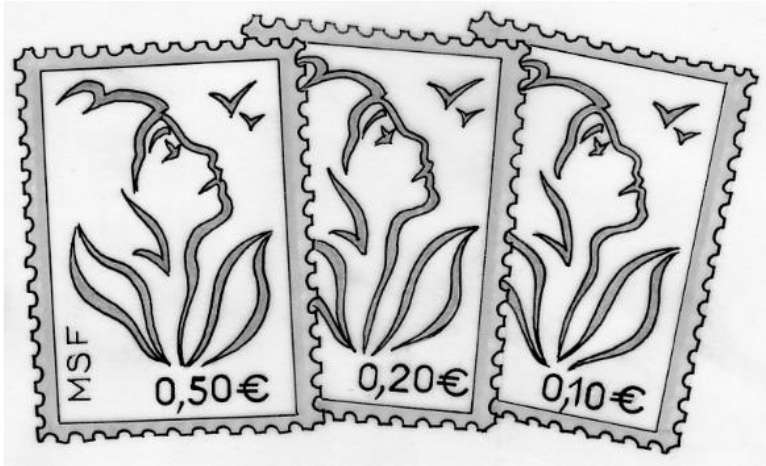
\includegraphics[width=0.4\linewidth]{figuras/MSFQ11}
	\end{figure}
\end{frame}

\begin{frame}[t]
	Sejam:
	\begin{description}
		\item[$ a $] total de selos de $\mathrm{R}\$ 0,10$
		\item[$ b $] total de selos de $\mathrm{R}\$ 0,20$
		\item[$ c $] total de selos de $\mathrm{R}\$ 0,50$
	\end{description}
	Sabemos que $ a,b,c\in\mathbb{Z}_+ $ e que:
	\begin{equation*}
		\begin{cases}
		0,1a+0,2b+0,5c=10\\
		a = 10b
		\end{cases}
	\end{equation*}
	Combinando as duas equações anteriores obtemos que:
	\begin{equation*}
		1,2b+0,5c=10 \implies c = 20-2,4b
	\end{equation*}
	Como $c\in\mathbb{Z}_+$ então:
	\begin{equation*}
		20-2,4b>0\implies b<8,333\ldots
	\end{equation*}
	Como $ b\in\mathbb{Z}_+ $ uma solução do problema é todo valor de $ b\in\{1,2,3,4,5,6,7,8\} $ tal que $a,c\in\mathbb{Z}_+$.
	A única solução possível é:
	\begin{equation*}
		b=5\implies
		\begin{cases}
		c = 8\\
		a = 50
		\end{cases}
	\end{equation*}
\end{frame}

\begin{frame}[t]
	\begin{exercicio}{Olimpíada Internacional Mathématiques Sans Frontières 2021 - Questão 12}
		Para dar uma volta completa em torno de uma ilha caribenha, Hassan leva uma hora em seu barco a remo, enquanto, Seema, sua amiga, gasta apenas 10 minutos com sua nova lancha.
		Os dois amigos partem de um mesmo lugar e seguem o mesmo caminho.
		Quando Hassan tiver completado uma volta, quantas voltas Seema terá dado?
		Quanto tempo Seema levara para encontrar Hassan novamente?
	\end{exercicio}
	\begin{figure}
		\centering
		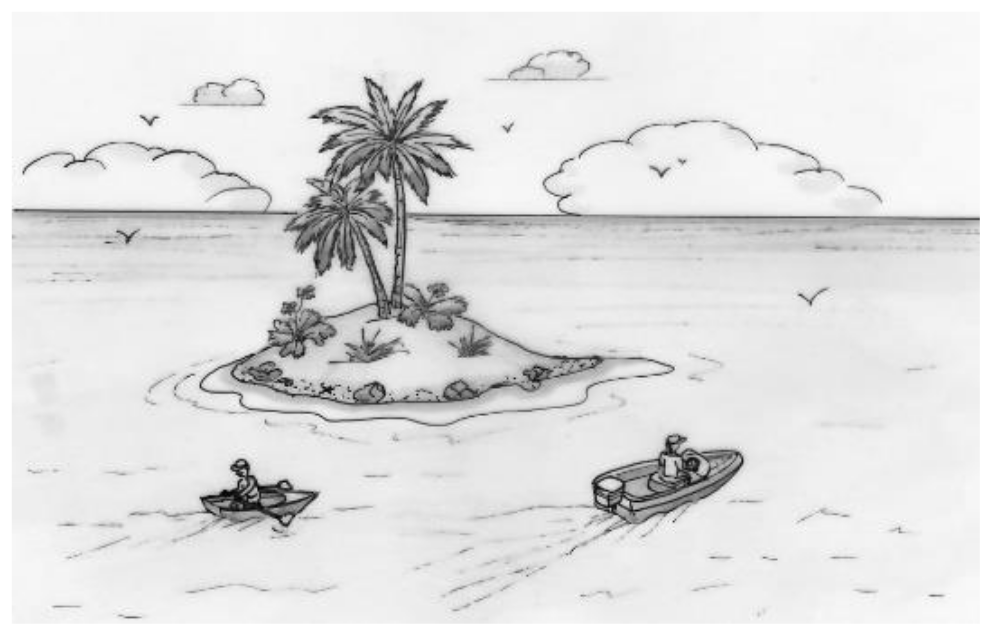
\includegraphics[width=0.55\linewidth]{figuras/MSFQ12}
	\end{figure}
\end{frame}

\begin{frame}[t]
	\begin{exercicio}{$ 37^{a} $ Olimpíada de Matemática da Unicamp - IMECC - Questão 2}
		Seja um triângulo equilátero de lado $L$.
		Vamos considerar a divisão do triângulo por retas paralelas a um dos lados (fixo).
		Considere a altura em relação à esse lado.
		Esta altura é dividida pelas retas paralelas em segmentos de altura $a_1>a_2>\cdots>a_n$.
		\begin{enumerate}[a]
			\item Se quisermos dividir o triângulo em 2 pedaços de mesma área, qual seria a altura $ a_1 $?
			\item Se quisermos dividir o triângulo em 3 pedaços de mesma área, quais seriam as alturas $a_1$ e $a_2$?
			\item Se quisermos dividir o triângulo em $ n $ pedaços de mesma área, quais seriam as alturas $a_1,a_2,\ldots a_{n-1}$?
			\item O que poderíamos falar sobre estas grandezas se o triângulo não for equilátero?
		\end{enumerate}
	\end{exercicio}
	\begin{figure}
		\centering
		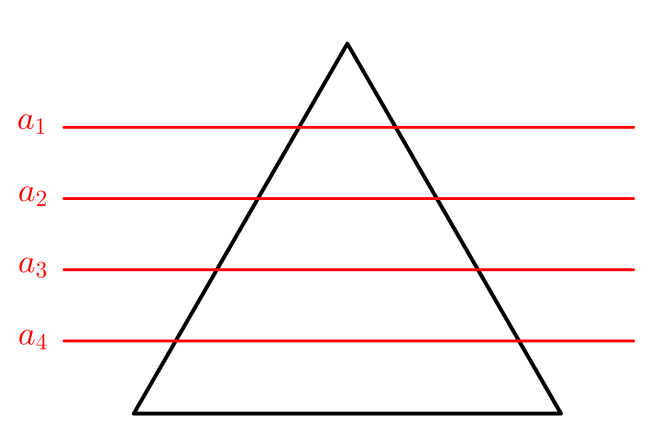
\includegraphics[width=0.3\linewidth]{figuras/OMUQ2}
	\end{figure}
\end{frame}

\end{document}
